\documentclass[12pt,a4letter]{article}
\usepackage[T2A]{fontenc}
\usepackage[utf8]{inputenc}
\usepackage[russian]{babel}
\usepackage{graphicx}
\usepackage{amsfonts}
\usepackage{indentfirst}
\usepackage{amsmath}
\usepackage{amsthm}
\usepackage{nicematrix}
\usepackage{hyperref}
\hypersetup{
    colorlinks=true,
    linkcolor=black,
    filecolor=magenta,      
    urlcolor=cyan,
    pdftitle={Lab3},
    pdfpagemode=FullScreen,
}
\usepackage{soulutf8}
\usepackage[left=1cm,right=1cm,
    top=2cm,bottom=2cm]{geometry}
\usepackage{titleps}
    \newpagestyle{main}{
        \setheadrule{0.4pt}
        \sethead{something}{\thepage}{}
}
%\pagestyle{main}
\theoremstyle{plain}
\newtheorem{theorem}{Теорема}[section]
\newtheorem{corollary}{Следствие}[theorem]
\newtheorem*{example}{\textit{Пример}}
\newtheorem*{definition}{Определение}

\begin{document}
\begin{titlepage}
    \newpage
    \begin{center}
        \begin{tabular}{cc}
            \parbox{12cm}{\centering \textbf{НИУ ИТМО}} \\
            \\
            \hline
            \hline
        \end{tabular}
    \end{center}

    \begin{center}
        \caps{\textbf{Факультет систем управления и робототехники}}\\
    \end{center}

    \vspace{1cm}

    \begin{center}
        \textsc{Лабораторная работа №6 \\ по дисциплине <<Техническое зрение>>}
    \end{center}

    \vspace{8em}

    \noindent Выполнили:  \hfill Гридусов Д.Д

    \vspace{20pt}

    \noindent Преподаватель: \hfill Шаветов С.В. \\
    \\
    \vfill

    \begin{center}
        Санкт-Петербург \\2024 г.
    \end{center}

\end{titlepage}

\tableofcontents
\newpage
\section{Введение}

\noindent \textbf{Цель работы:} Освоение принципов математической морфологии в области обработки и анализа изображений.
\\
\noindent \textbf{Теоритическое обоснование}
\\
\noindent Морфология - наука о форме. Методы морфологического анализа – это методы решения задач
узнавания, классификации объектов, оценки параметров объектов,
выделения различия в сценах по их изображениям (сигналам). Основаны
на понятии формы сигнала. Математическая же морфология (долгое время эти две морфологии считались разными) основана на теории множеств. Чтобы использовать морфологию для анализа изображений вводятся морфологические фильтры - множество операторов, являющихся равносильными и увеличивающими. А также морфологические операции на бинарных изображениях (вычитание и сложение Минковского), которые позволяют используя структурный элемент ввести основные операции: дилатацию изображения и эрозию.
\section{Исправить изображение морфологией}
\noindent Возьмем два изображения: пиксельный инь и янь, и какую-то карточку. В первом случае будем пытаться убрать деление на пиксели (применим операцию открытия). А во втором случае будем решать насущную проблему - авторское право. Применив последовательно открытие и закрытие попробуем убрать надпись в правом нижнем углу.

\begin{figure}[!htb]
    \minipage{0.5\textwidth}
    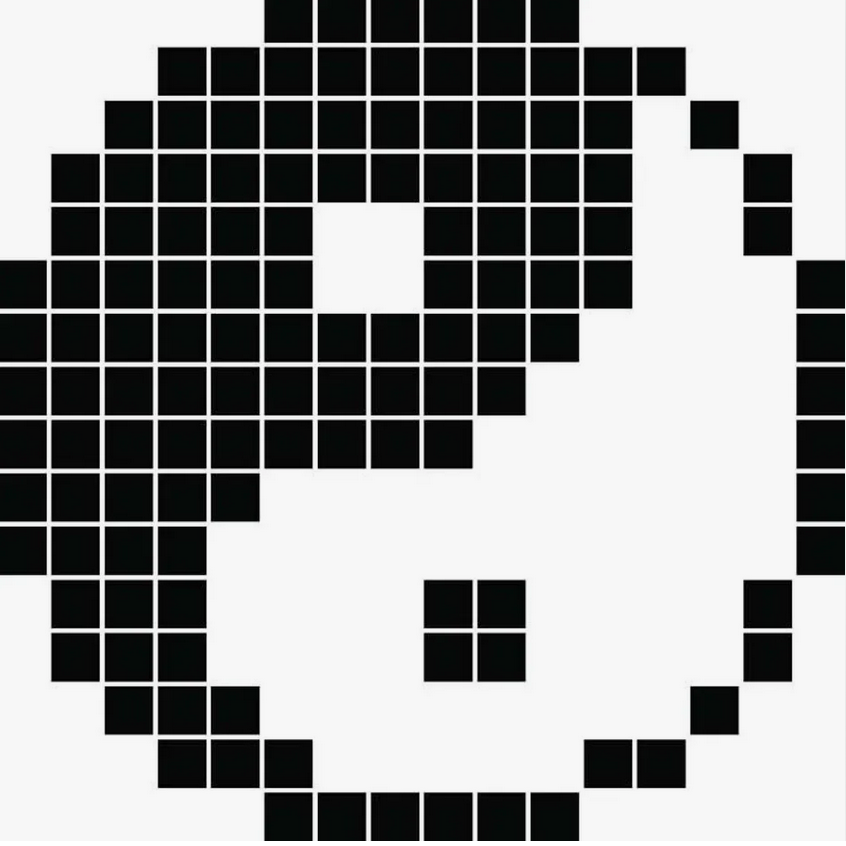
\includegraphics[width=\linewidth]{../img/original/1.png}
    \caption{Исходное изображение 1}
    \endminipage\hfill
    \minipage{0.5\textwidth}
    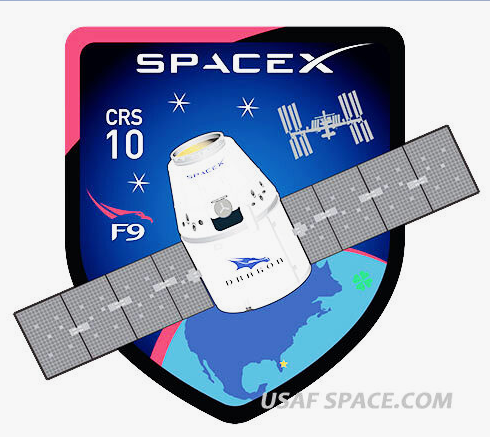
\includegraphics[width=\linewidth]{../img/original/2.png}
    \caption{Исходное изображение 2}
    \endminipage\hfill
\end{figure}

\newpage


\begin{figure}[!htb]
    \minipage{0.5\textwidth}
    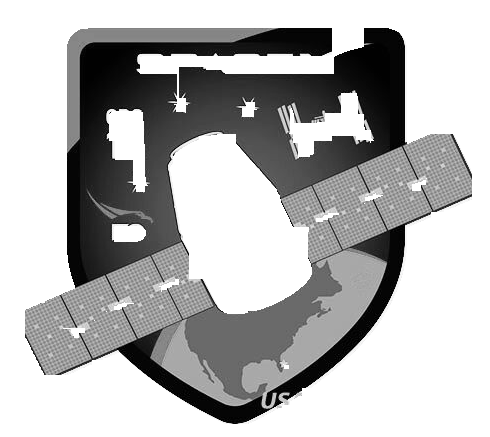
\includegraphics[width=\linewidth]{../img/outputs/morph_filters/spacex_only_close.png}
    \caption{Только закрытие}
    \endminipage\hfill
    \minipage{0.5\textwidth}
    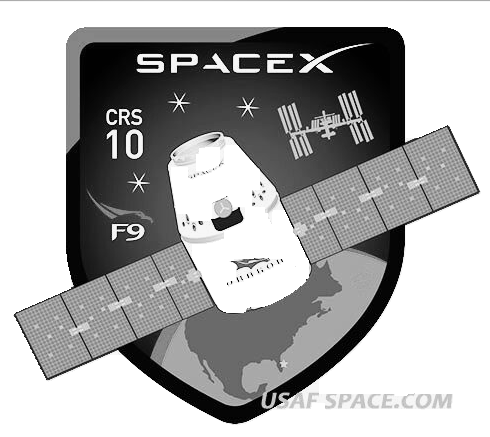
\includegraphics[width=\linewidth]{../img/outputs/morph_filters/spacex_only_open.png}
    \caption{Только открытие}
    \endminipage\hfill
\end{figure}

\begin{figure}[!htb]
    \minipage{0.5\textwidth}
    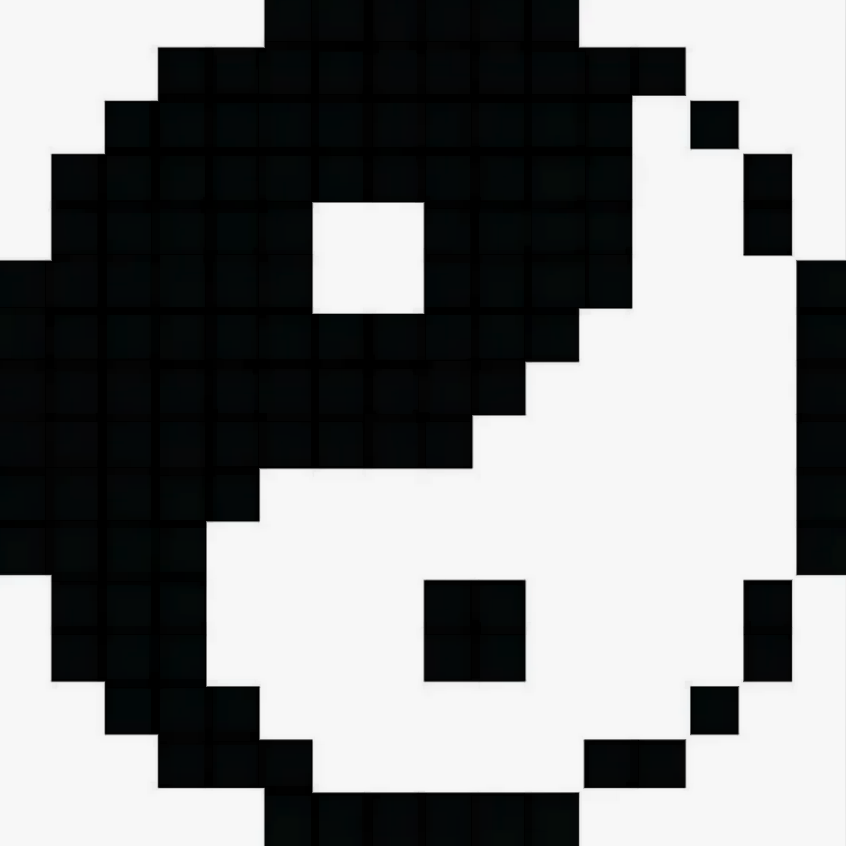
\includegraphics[width=\linewidth]{../img/outputs/morph_filters/pixel_erode_dilate.png}
    \caption{Открытие первого}
    \endminipage\hfill
    \minipage{0.5\textwidth}
    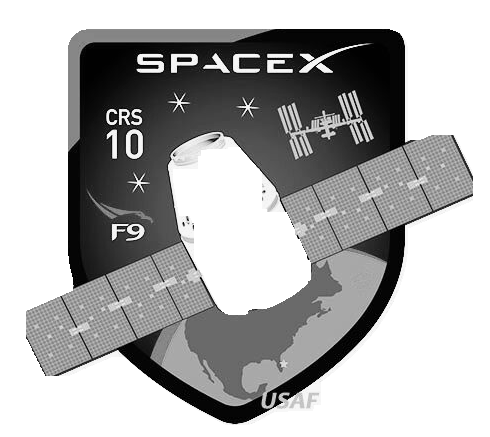
\includegraphics[width=\linewidth]{../img/outputs/morph_filters/spaceX_open_close.png}
    \caption{Открытие + закрытие второго}
    \endminipage\hfill
\end{figure}

\noindent После некоторого подбора параметров цели были достигнуты (ну, почти) - инь и янь теперь не настолько пиксельно выглядит (убрали внутренние дырки). А с карточкой сложнее - мы убрали большую часть надпись (осталась только та, что примыкает к изображению), но пожертвовали частью информации на карточке.
\newpage
\section{Разделение объектов}
\noindent \textbf{Листинг 3.1} Разделение объектов, выделение границ
\begin{lstlisting}

cv::Mat create_mask(cv::Mat img)
{
    cv::Mat img_gray, img_thresholded;
    cv::cvtColor(img, img_gray, cv::COLOR_BGR2GRAY);
    cv::threshold(img_gray, img_thresholded, 84, 255, cv::THRESH_BINARY_INV);
    cv::Mat B = cv::getStructuringElement(cv::MORPH_ELLIPSE, cv::Size(7, 7));


    cv::Mat BW2;
    cv::morphologyEx(img_thresholded, BW2, cv::MORPH_ERODE, 
    B, cv::Point(-1, -1), 14, cv::BORDER_CONSTANT, cv::Scalar(0));
    cv::Mat D, C, S;
    cv::Mat T = cv::Mat::zeros(img_thresholded.size(), img_thresholded.type());
    int pix_num = img_thresholded.rows * img_thresholded.cols;
    while (cv::countNonZero(BW2) < pix_num)
    {

        cv::morphologyEx(BW2, D, cv::MORPH_DILATE, 
        B, cv::Point(-1, -1), 1,
        cv::BORDER_CONSTANT, cv::Scalar(0));

        cv::morphologyEx(D, C, cv::MORPH_CLOSE,
        B, cv::Point(-1, -1), 1,
        cv::BORDER_CONSTANT, cv::Scalar(0));

        S = C - D;
        cv::bitwise_or(S, T, T);
        BW2 = D;
    }

    cv::morphologyEx(T, T, cv::MORPH_CLOSE, B, cv::Point(-1, -1), 14, cv::BORDER_CONSTANT, cv::Scalar(255));
    cv::bitwise_and(~T, img_thresholded, img_thresholded);

    return img_thresholded;

}


cv::Mat find_borders(cv::Mat img)
{
    cv::Mat img_gray, img_thresholded;
    cv::cvtColor(img, img_gray, cv::COLOR_BGR2GRAY);
    cv::threshold(img_gray, img_thresholded, 80, 255, cv::THRESH_BINARY_INV);
    
    cv::Mat img_erode;
    cv::Mat B = cv::getStructuringElement(cv::MORPH_ELLIPSE, cv::Size(3, 3));
    cv::erode(img_thresholded, img_erode, B, cv::Point(-1, -1), 1);
    cv::Mat border;
    border = img_thresholded - img_erode;
    return border;
}

\end{lstlisting}

\begin{figure}[!htb]
    \minipage{0.5\textwidth}
    
\includegraphics[width=\linewidth]{../img/original/3.png}
    \caption{Исходное изображение}
    \endminipage\hfill
    \minipage{0.5\textwidth}
    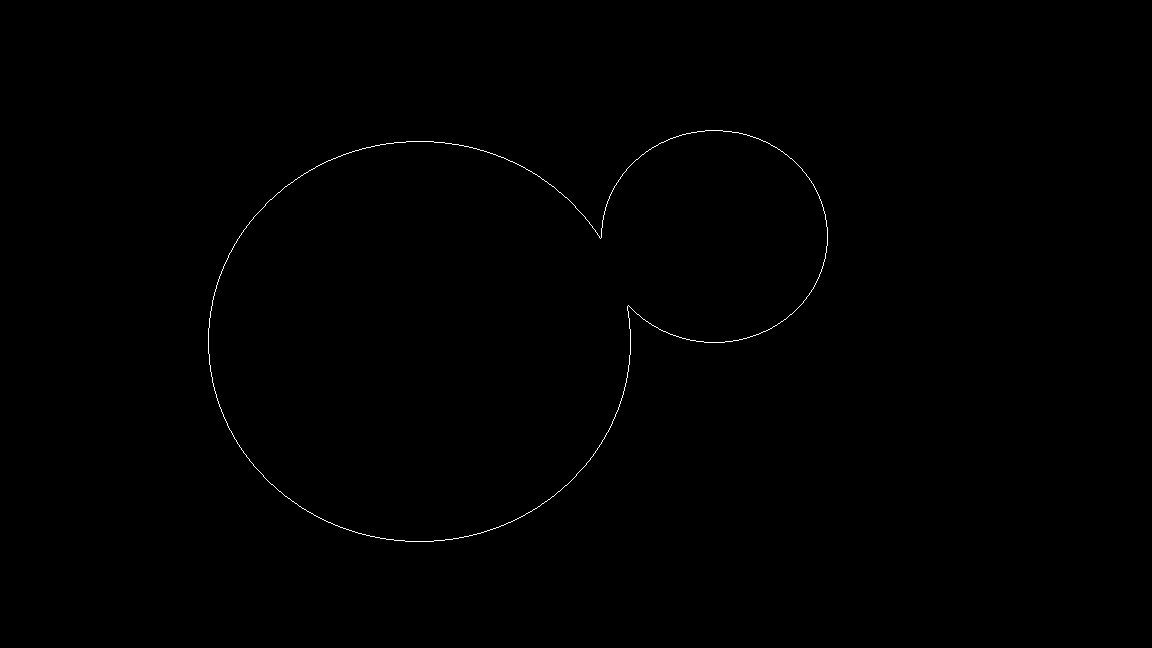
\includegraphics[width=\linewidth]{../img/outputs/divide_objects/border_img.jpg}
    \caption{Исходная граница}
    \endminipage\hfill
\end{figure}


\begin{figure}[!htb]
    \minipage{0.45\textwidth}
    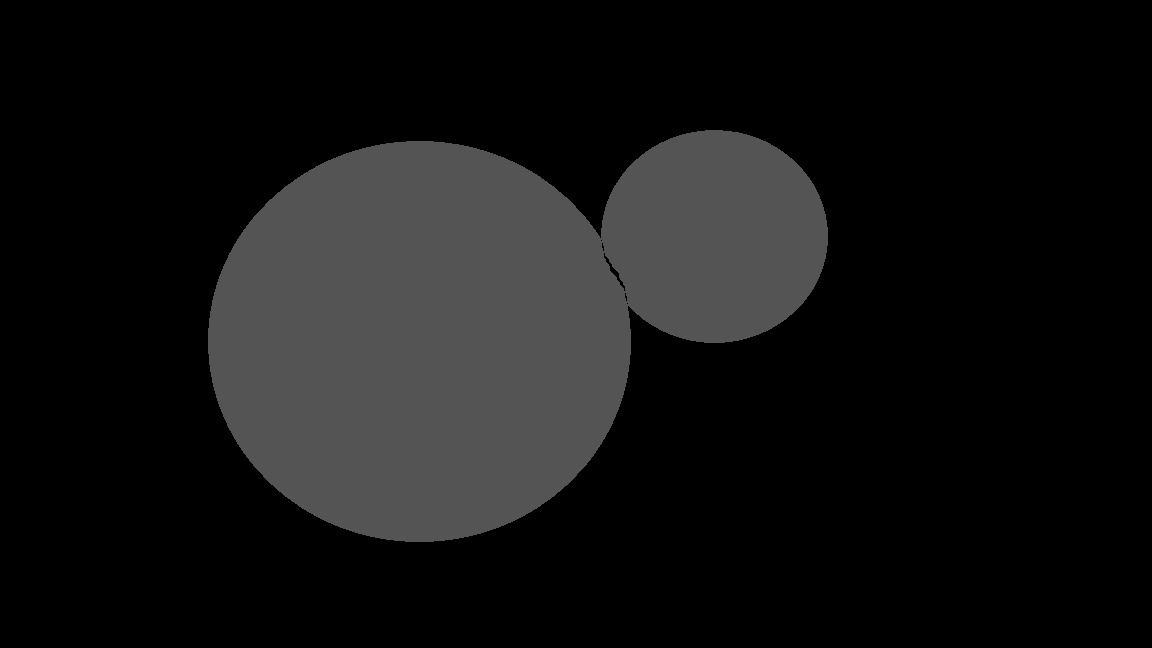
\includegraphics[width=\linewidth]{../img/outputs/divide_objects/img_divided.jpg}
    \caption{Разделенные объекты}
    \endminipage\hfill
    \minipage{0.45\textwidth}
    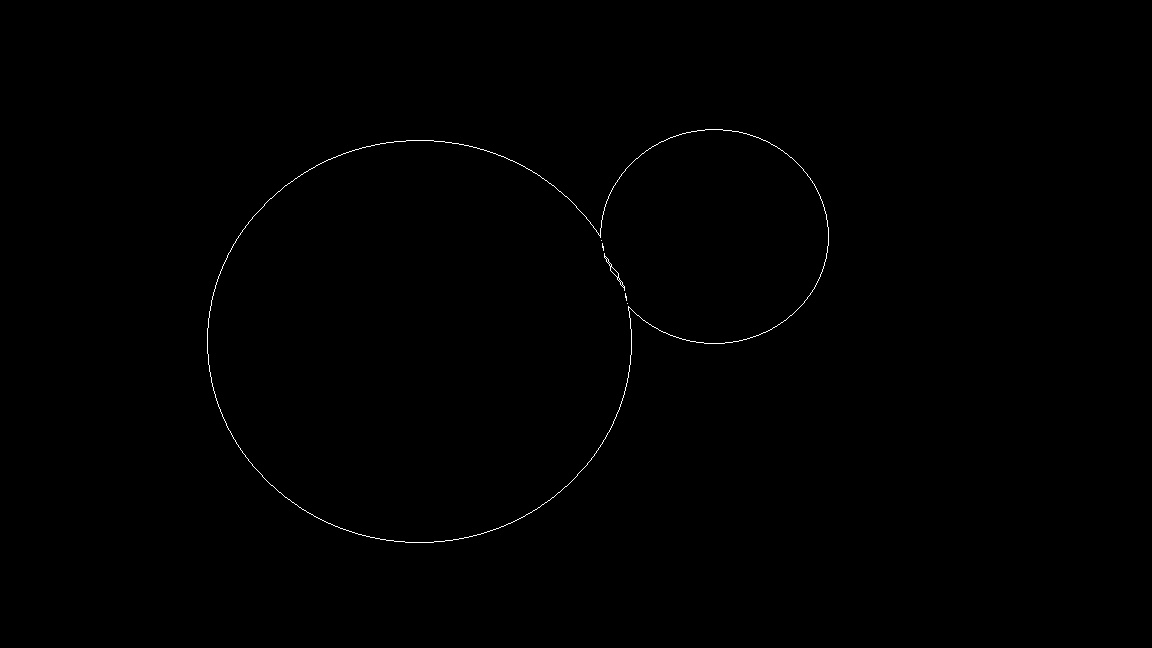
\includegraphics[width=\linewidth]{../img/outputs/divide_objects/borders_divided.jpg}
    \caption{Новая граница}
    \endminipage\hfill
\end{figure}

\noindent В этом пункте мы рассмотрели применение морфологических фильтров сразу для двух целей: разделения объектов и выделения их границ. Все получилось достаточно успешно, кроме этапа подбора изображния - пришлось переключаться на Windows и вспоминать  кто такой Paint (ни одной работы без того, чтобы пожаловаться - ужас).
\section{Сегментация методом управляемого водораздела}
\noindent \textbf{Листинга 4.1} Метод управляемого водораздела
\begin{lstlisting}
cv::Mat segmentation_watershed(cv::Mat img)
{
    cv::Mat img_gray, img_bw;
    cv::cvtColor(img, img_gray, cv::COLOR_BGR2GRAY);
    cv::threshold(img_gray, img_bw, 0, 255, cv::THRESH_BINARY + cv::THRESH_OTSU);
    bwareaopen(img_bw, img_bw, 10, 4);

    cv::Mat B = cv::getStructuringElement(cv::MORPH_ELLIPSE, cv::Size(11, 11));
    cv::morphologyEx(img_bw, img_bw, cv::MORPH_CLOSE, B);

    cv::Mat img_fg;
    double img_fg_min, img_fg_max;
    cv::distanceTransform(img_bw, img_fg, cv::DIST_L2, 5);
    cv::minMaxLoc(img_fg, &img_fg_min, &img_fg_max);
    cv::threshold(img_fg, img_fg, 0.6 * img_fg_max, 255, 0);
    img_fg.convertTo(img_fg, CV_8U, 255.0 / img_fg_max);  
    cv::Mat markers;
    int num = cv::connectedComponents(img_fg, markers);

    cv::Mat img_bg=cv::Mat::zeros(img_bw.size(), img_bw.type());
    cv::Mat markers_bg=markers.clone();
    cv::watershed(img, markers_bg);
    img_bg.setTo(cv::Scalar(255), markers_bg==-1);

    cv::Mat img_unk;
    cv::bitwise_not(img_bg, img_unk);
    cv::subtract(img_unk, img_fg, img_unk);

    markers += 1;
    markers.setTo(cv::Scalar(0), img_unk == 255);
    cv::watershed(img, markers);

    cv::Mat markers_jet;
    markers.convertTo(markers_jet, CV_8U, 255.0/(num+1));
    cv::applyColorMap(markers_jet, markers_jet, cv::COLORMAP_JET);

    img.setTo(cv::Scalar(255, 255, 0), markers==-1);
    return img;
}

void bwareaopen(const cv::Mat &A, cv::Mat &C, int dim, int conn)
{
    if (A.channels() != 1 && A.type() != A.type() != CV_8U && A.type() != CV_32F)
    {
        return;
    }

    cv::Mat labels, stats, centers;
    int num = cv::connectedComponentsWithStats(A, labels, stats, centers, conn);

    C = A.clone();
    std::vector<int> td;
    for (int i = 0; i < num; i++)
    {
        if (stats.at<int>(i, cv::CC_STAT_AREA) < dim)
        {
            td.push_back(i);
        }
    }
    if (td.size() > 0)
    {
        if (A.type() == CV_8U)
        {
            for (int i = 0; i < C.rows; i++)
            {
                for (int j = 0; j < C.cols; j++)
                {
                    for (int k = 0; k < td.size(); ++k)
                    {
                        if (labels.at<int>(i, j) == td[k])
                        {
                            C.at<uchar>(i, j) = 0;
                            continue;
                        }
                    }
                }
            }
        }
        else
        {
            for (int i = 0; i < C.rows; i++)
            {
                for (int j = 0; j < C.cols; j++)
                {
                    for (int k = 0; k < td.size(); k++)
                    {
                        if (labels.at<int>(i, j) == td[k])
                        {
                            C.at<float>(i, j) = 0;
                            continue;
                        }
                    }
                }
            }
        }
    }
}

\end{lstlisting}


\begin{figure}[!htb]
    \minipage{0.5\textwidth}
    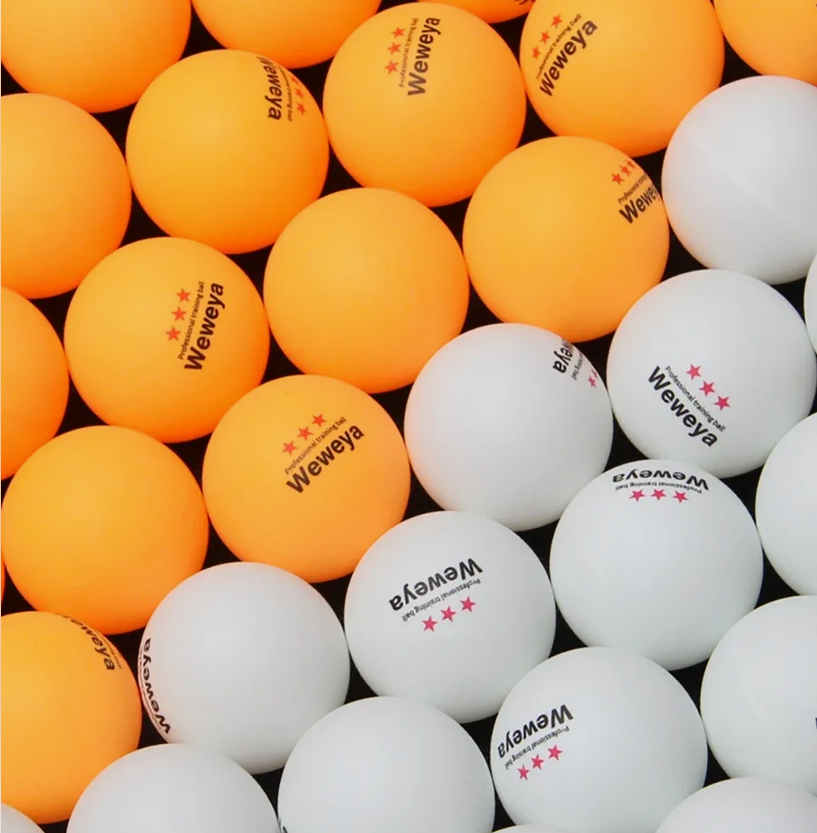
\includegraphics[width=\linewidth]{../img/original/balls.png}
    \caption{Оригинальное изображения}
    \endminipage\hfill
    \minipage{0.5\textwidth}
    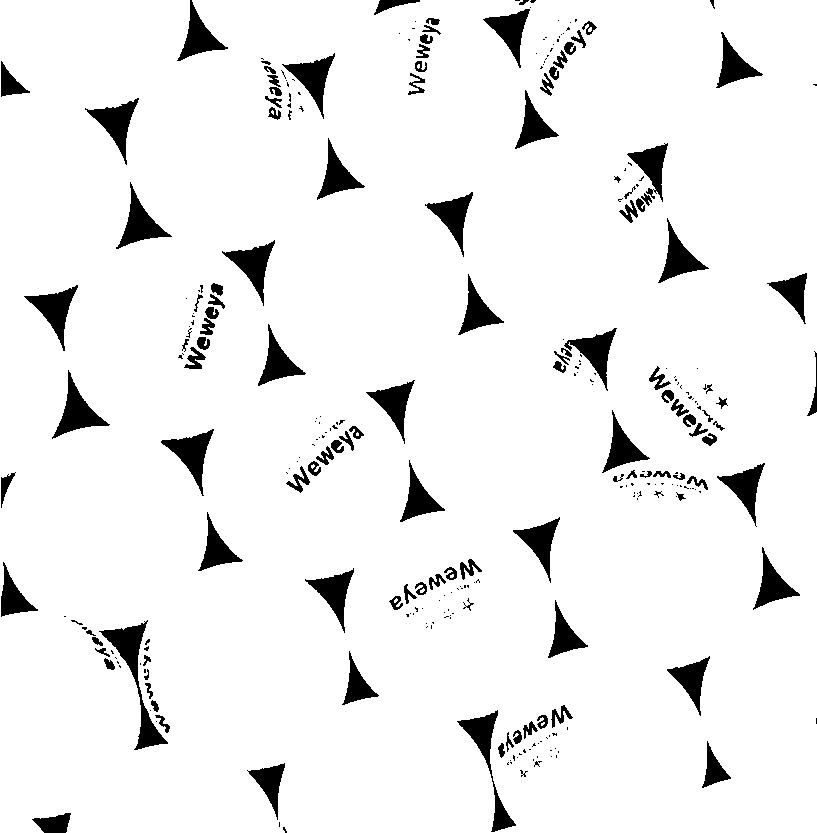
\includegraphics[width=\linewidth]{../img/outputs/segmentation_watershed/balls_bwearopen.png}
    \caption{Бинаризация + bwearopen}
    \endminipage\hfill
\end{figure}
\newpage
\begin{figure}[!htb]
    \minipage{0.5\textwidth}
    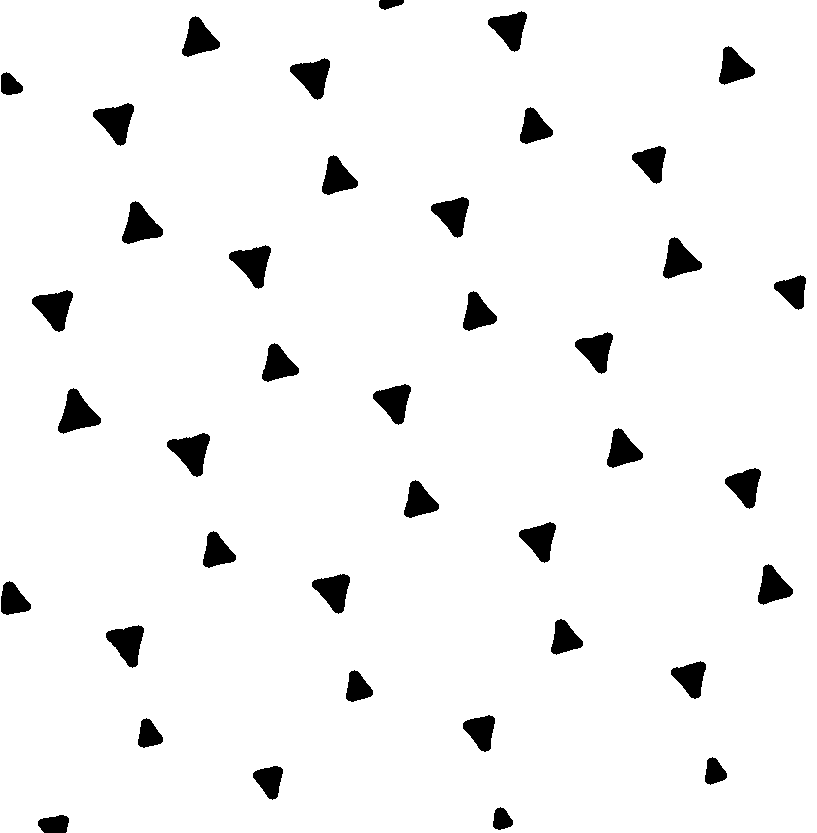
\includegraphics[width=\linewidth]{../img/outputs/segmentation_watershed/balls_close.png}
    \caption{MORPH\_CLOSE}
    \endminipage\hfill
    \minipage{0.5\textwidth}
    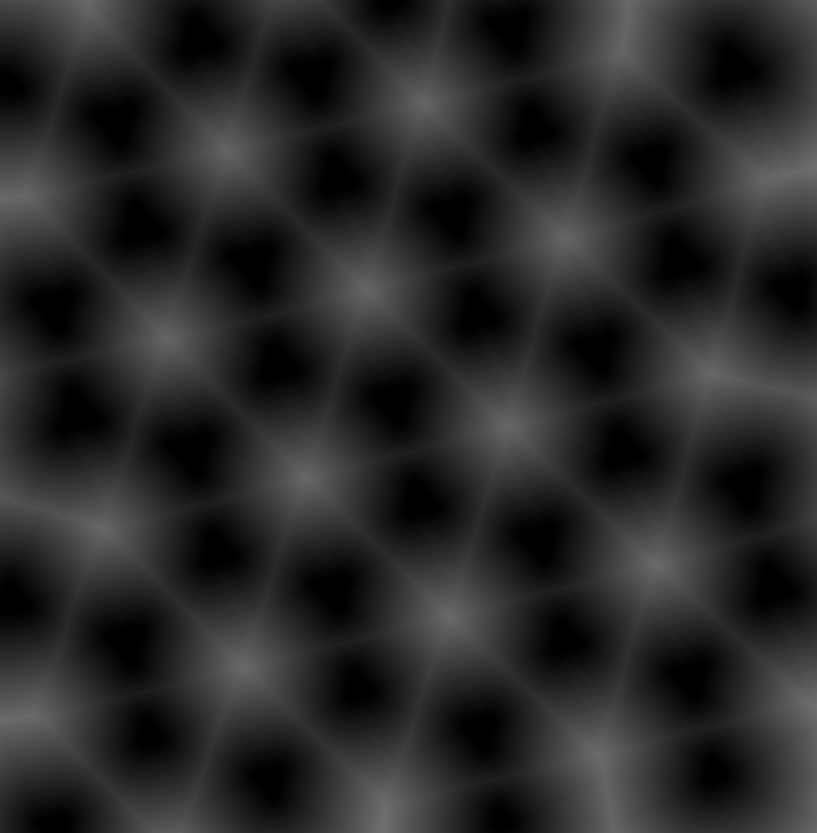
\includegraphics[width=\linewidth]{../img/outputs/segmentation_watershed/balls_dist.png}
    \caption{Преобразование L2 метрики}
    \endminipage\hfill
\end{figure}

\begin{figure}[!htb]
    \minipage{0.5\textwidth}
    
\includegraphics[width=\linewidth]{../img/outputs/segmentation_watershed/balls_front_markers.png}
    \caption{Макеры переднего плана}
    \endminipage\hfill
    \minipage{0.5\textwidth}
    
\includegraphics[width=\linewidth]{../img/outputs/segmentation_watershed/balls_back_markers.png}
    \caption{Маркеры заднего плана}
    \endminipage\hfill
\end{figure}
\newpage
\begin{figure}[!htb]
    \minipage{0.5\textwidth}
    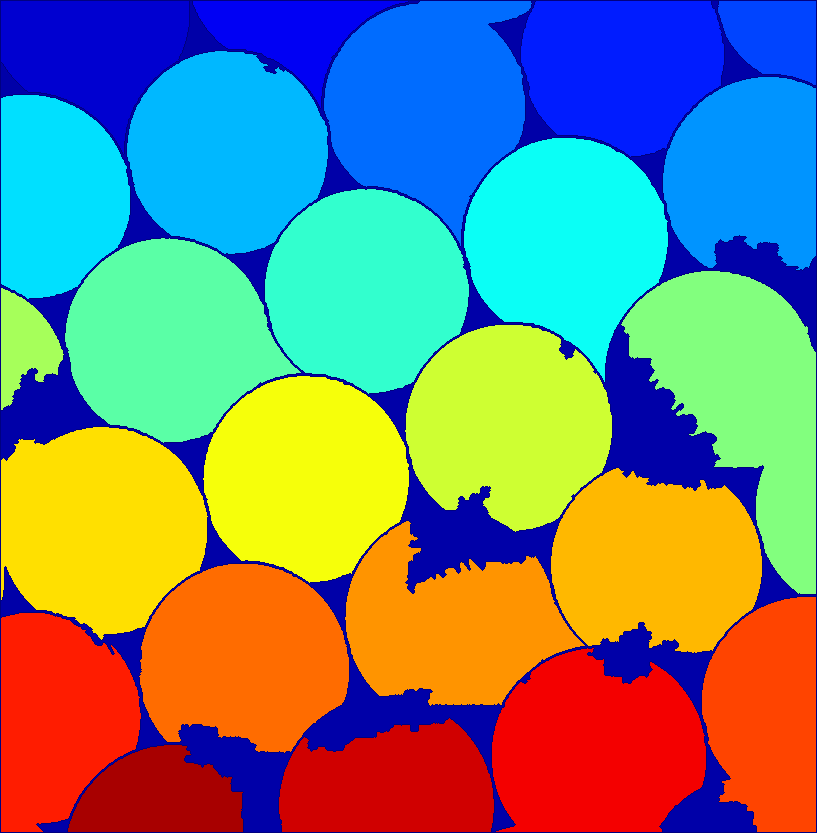
\includegraphics[width=\linewidth]{../img/outputs/segmentation_watershed/balls_segmentation.png}
    \caption{Сегментация}
    \endminipage\hfill
    \minipage{0.5\textwidth}
    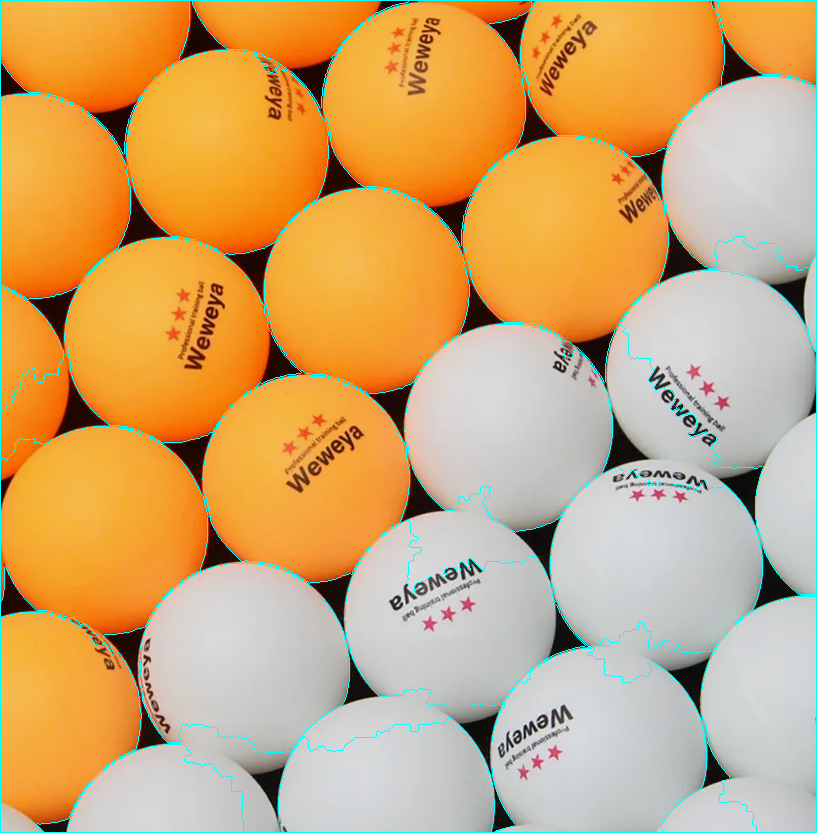
\includegraphics[width=\linewidth]{../img/outputs/segmentation_watershed/balls.png}
    \caption{Сегментированное изображение}
    \endminipage\hfill
\end{figure}

\noindent Алгоритм работает очень даже неплохо, но важно правильно подобрать параметры (размер структурного элемента, количетсво повторений в методе morphologyEx).
\newpage 
\section{Эпилог}
\noindent \textbf{Вывод:} я освоил основные принципы математической морфологии в области обработки и анализа изображений. Действительно, появилось какое-то понимание, что это за методы, когда их применять. Что не может не радовать - я сдал эту работу в дедлайн (даже заранее, можно сказать). Курс был интересным и насыщенным, C++ - one love, спасибо!
\\
\noindent \textbf{Ответы на вопросы}
\begin{enumerate}
    \item Судя по экспериментальным данным и примеру из лекции - нет, не содержит.
    \item Необходимо использовать закрытие (дилатация + эрозия)
    \item Нужно из объекта убрать его эрозию
    \item Наука о форме, применяемая во многих областях. В анализе изображений позволяет решать, например, задачи узнавания и классификации.
\end{enumerate}
\end{document}